\chapter{System Models}
\label{chap:sys}
This chapter will outline the system models of flow-based biochips. We use the biochip architecture model and the biochemical application model used is proposed in \cite{wajid}. An extension to this biochip architecture model is proposed by the addition of fault-tolerant components and a fault model. Lastly the problem of application mapping will be described.

\section{Biochip Architecture Model}
The biochip architecture model is composed of three models: component model, architecture model and fault model. The following subsections will explain these models.

\subsection{Component Model}
In \cite{wajid}, a dual-layer component modeling framework is proposed consisting of a \emph{flow layer model} and a \emph{control layer model}. The flow layer model ($\mathcal{P}, C, H$) of each component $\mathcal{M}$, is characterised by a set of operational phases $\mathcal{P}$, the execution time C and the geometrical dimensions $H$. The control layer model captures the valve actuation details required for the on-chip execution of all operational phases of a component. 

The component library $\mathcal{L} = \mathcal{M}(\mathcal{P}, C, H)$ is shown in \autoref{tab:component-library}. The component library describes the set of components that a biochip architecture can have. The geometrical dimensions $H$ are given as length$\times$width and are scaled with a unit length being equal to 150$\mu m$. Therefore a length of 10 in \autoref{tab:component-library} corresponds to 1500$\mu m$. FT is an abbreviation for Fault-Tolerant. Considering \autoref{tab:component-library} the only change from a component to its fault-tolerant version is in width, however this is not the case. The introduction of fault-tolerant components is the difference between \autoref{tab:component-library} and the component library given in \cite{wajid}. The components and their fault-tolerant counterpart will be described in this section.

\begin{table}[H]
\centering
\caption{Component Library ($\mathcal{L}$): Flow Layer Model}
\begin{tabular}{| c | c | c | c |}
\hline
\textbf{Component} & \textbf{Phases($\mathcal{P}$)} & \textbf{$C$} & \textbf{$H$} \\ \hline
Mixer & Ip1 / Ip2 / \textbf{Mix} / Op1 / Op2 & 0.5 s & 30 $\times$ 30\\ \hline
FT-Mixer & Ip1 / Ip2 / \textbf{Mix} / Op1 / Op2 & 0.5 s &  30 $\times$ 30 \\ \hline
Filter & Ip /  \textbf{Filter} / Op1 / Op2 & 20 s& 120 $\times$ 30 \\ \hline
FT-Filter & Ip /  \textbf{Filter} / Op1 / Op2 & 20 s& 120 $\times$ 60 \\ \hline
Detector & Ip / \textbf{Detect} / Op & 5 s & 20 $\times$ 20 \\ \hline
FT-Detector & Ip / \textbf{Detect} / Op & 5 s & 20 $\times$ 40 \\ \hline
Separator & Ip1 / Ip2 / \textbf{Separate} / Op1 / Op2 & 140 s & 70 $\times$ 20 \\ \hline
FT-Separator & Ip1 / Ip2 / \textbf{Separate} / Op1 / Op2 & 140 s & 70 $\times$ 40 \\ \hline
Heater & Ip / \textbf{Heat} / Op & $20^{\circ}$ C/s & 40 $\times$ 15\\ \hline
FT-Heater & Ip / \textbf{Heat} / Op & $20^{\circ}$ C/s & 40 $\times$ 30 \\ \hline
Storage & Ip or Op & - & 90 $\times$ 30 \\ \hline
FT-Storage & Ip or Op & - & 90 $\times$ 40 \\ \hline
Metering & Ip / \textbf{Met} / Op1 / Op2 & - & 30 $\times$ 15 \\ \hline
Multiplexer & Ip or Op & - & 30 $\times$ 10 \\ \hline
\end{tabular}
\label{tab:component-library}
\end{table}

\subsubsection{Fault-tolerant Switch}
\autoref{fig:switch}a shows switches formed by combining valves. A switch can consist of one valve that restricts or allows flow in a channel or a switch can consist of more than one valve \cite{wajid}. Multiple valve switches are present at channel junctions and are used to control the path of the fluids entering the switch from different sides. The conceptual view of a switch is shown below the actual component design. A switch can fail in different ways. Each valve in the switch can be stuck open or stuck closed. For example, if valve $v_3$ in the third switch with four valves is stuck closed the effect is that fluid is restricted from entering the switch from the channel controlled by $v_3$ and the fluid is restricted from leaving the switch going to the channel controlled by $v_3$. However if the valve $v_3$ is stuck open, the fluid is allowed to enter the switch from the channel controlled by $v_3$ and leave the switch going to any other channel. But if the fluid is entering the switch from any other valve ($v_1$, $v_2$ or $v_4$) than $v_3$, the fluid can only leave the switch going to the channel controlled by $v_3$.
\begin{figure}
\centering
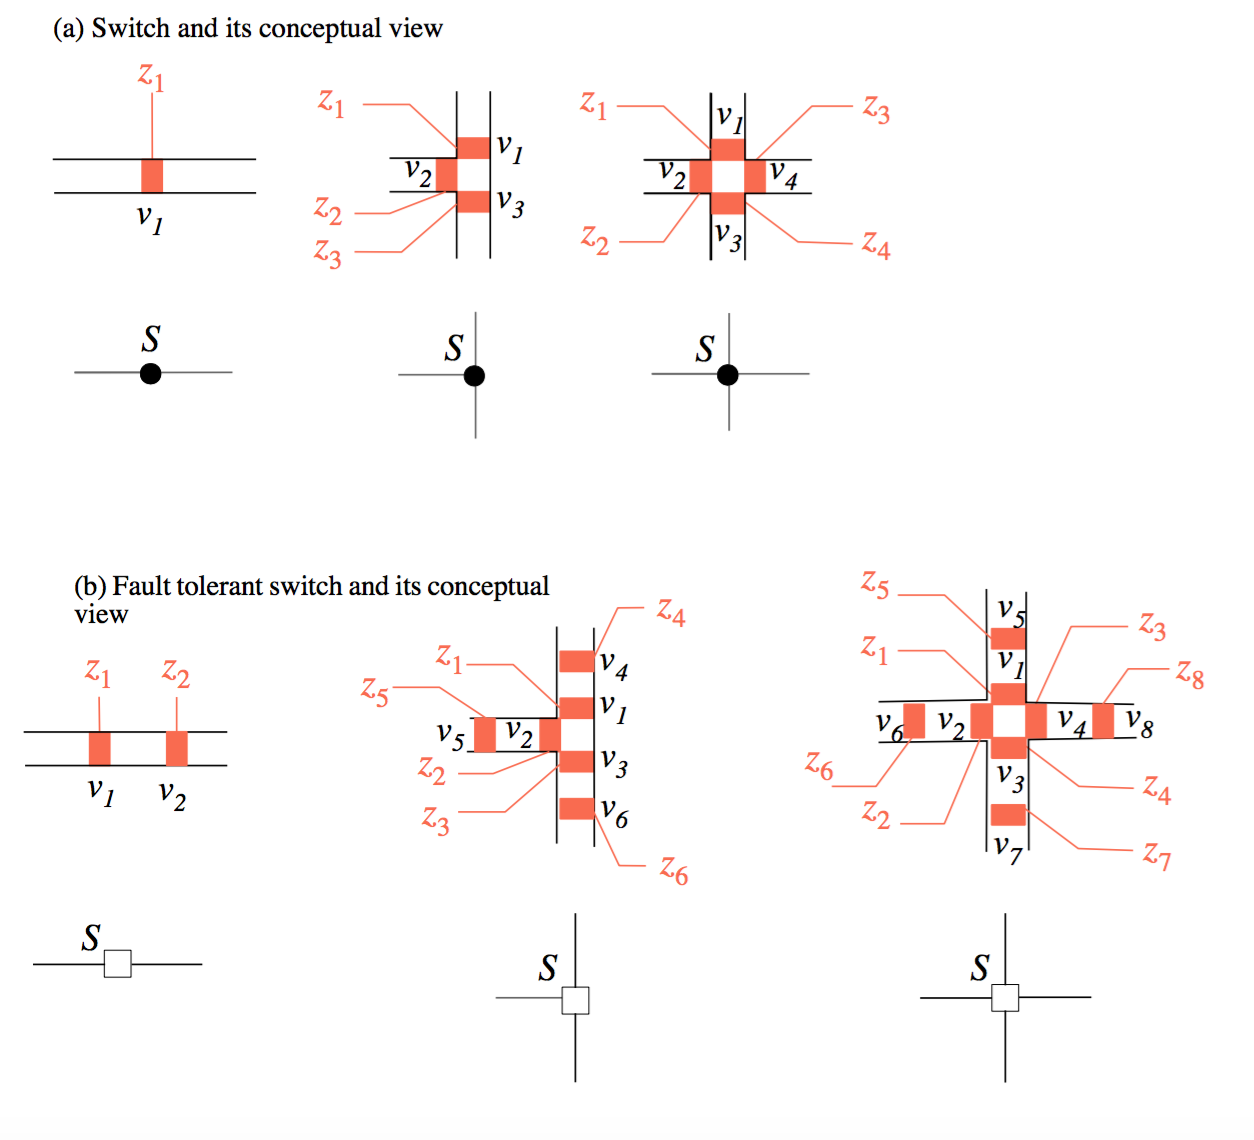
\includegraphics[scale=0.4]{figures/switch.png}
\caption[Switch and fault-tolerant switch]{Switch and fault-tolerant switch}
\label{fig:switch}
\end{figure}

\autoref{fig:switch}b shows the fault tolerant version of each switch in \autoref{fig:switch}a. These are called fault-tolerant switches or \emph{ft-switches} for short. The ft-switch is formed by combining valves as regular switches and function like regular switches. The conceptual view of a ft-switch is shown below the actual component design. A ft-switch has an extra added valve for each valve in a regular switch. The ft-switch tolerates faults that causes the valves to be stuck open as the extra added valve can compensate for the failing valve. However, if a valve is stuck closed, the switch is still faulty and the fluid is still restricted from leaving the switch to the channel the valve controls, and from entering the switch from that channel. A switch cannot consist of more than 4 valves, i.e. it cannot restrict / allow flow in more than 4 channels. This also applies for the ft-switch however the maximum number of valves is 8, but it cannot restrict / allow flow in more than 4 channels. This is due to cleaning difficulties and for the reason that fluid can be trapped inside the switch if it has more valves (i.e. channels).


\subsubsection{Fault-tolerant Mixer}
\autoref{fig:mixer}a shows a pneumatic mixer, which is implemented by nine microfluidic valves, $v_1$ to $v_9$. \autoref{fig:mixer}b shows the conceptual view of the same mixer. The valve set $\{v_4, v_5, v_6\}$ works as on-chip pump which is used to perform the mixing. The valve set $\{v_1, v_2, v_3\}$ is termed as switch $S_1$ and facilitates the inputs. The valve set $\{v_7, v_8, v_9\}$ is termed as switch $S_2$ and facilitates the outputs. The mixer has five operational phases. The first two phases represent the input of two fluid samples to be mixed, which is followed by the mixing phase. The mixed sample is then transported out of the mixer in the last two phases. The mixer can fail in various ways. Each valve in the mixer can be stuck closed or stuck open. The two channels inside the mixer can also fail as both channels can suffer from a block defect or a leakage. For example, any valve in the valve-set $\{v_4, v_5, v_6\}$, that acts as the pump can suffer from being stuck open or closed and the mixer will therefore not be able to perform its mixing operation. 
\begin{figure}
\centering
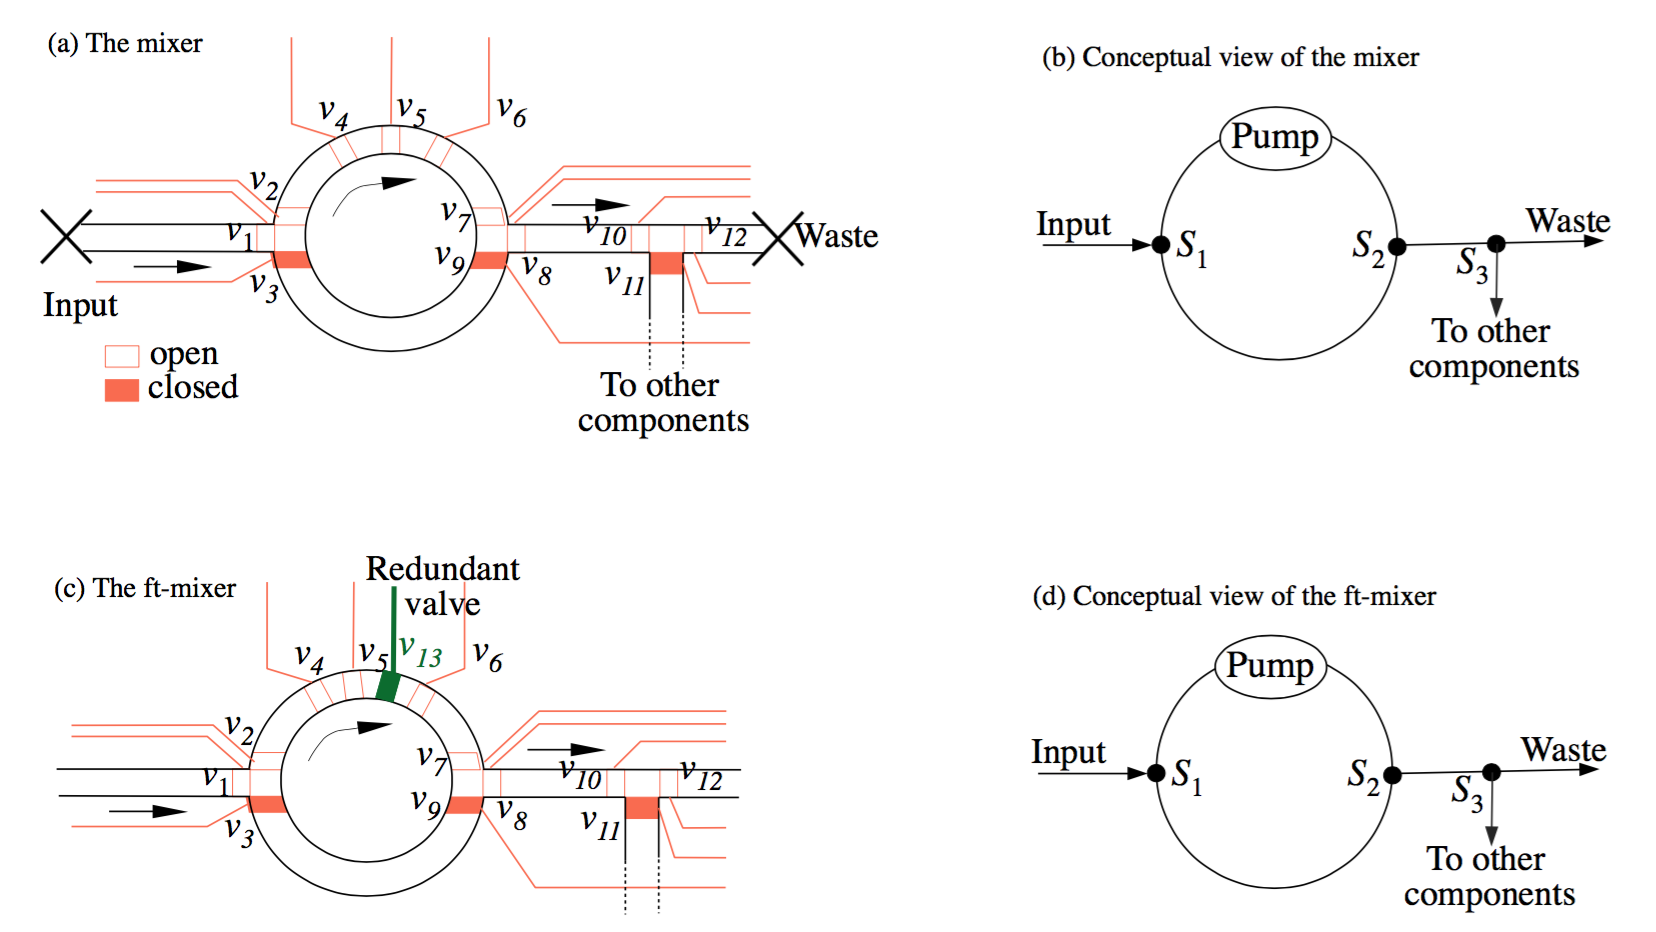
\includegraphics[scale=0.4]{figures/mixer-and-ftmixer.png}
\caption[Mixer and fault-tolerant mixer]{Mixer and fault-tolerant mixer}
\label{fig:mixer}
\end{figure}

\autoref{fig:mixer}c shows a fault-tolerant version of the pneumatic mixer called fault-tolerant mixer or \emph{ft-mixer} for short. \autoref{fig:mixer}d shows the conceptual view of the same ft-mixer. The ft-mixer has the same operational phases as the regular mixer and performs them in the same way. The difference is the added valve $v_{13}$. The purpose of this valve is to tolerate the fault of any valve in the pump being stuck open. In case, any of the valves in the pump are stuck open, the pump will still be functional by virtue of $v_{13}$ and the mixing can still be performed. However, in case, any of the other possible faults discussed previously happen, the ft-mixer will not be able to perform the mixing operation. It is possible to have a pump consisting of four valves as long as the amount of space between the valves is kept small, i.e. the valves should be close together to perform the pumping action. The result is that the pump can still function as intended and thereby perform the mixing.

It is possible to route through the mixers as valves are controlling its mixing operation. The valves are opened and closed by the designer. Therefore, the fluid can be routed through the mixer without being unintentionally affected by a mixing operation. Additionally, it is possible to route through the mixers even with faults affecting it. For example, if the mixer suffers from a blocked channel ($v_3$-$v_9$), the mixing operation cannot be performed, but it can use the other non-faulty channel ($v_2$ to $v_7$) to route through the mixer. Furthermore, it is possible for the mixer to receive input from both sides and similarly send output to both sides.


\subsubsection{Fault-tolerant Heater, Filter, Detector and Separator}
This section outlines the components heater, filter, detector, separator and their fault-tolerant counterparts. These components are similar in the sense that they consist only of a channel where the channel has a specific operational functionality. The functionality is the only thing that differs between the components. Therefore \autoref{fig:comp-and-ftcomp} will be explained first with the possible faults and the introduced fault-tolerant component. Afterwards the details specific to each component will be described.

\begin{figure}
\centering
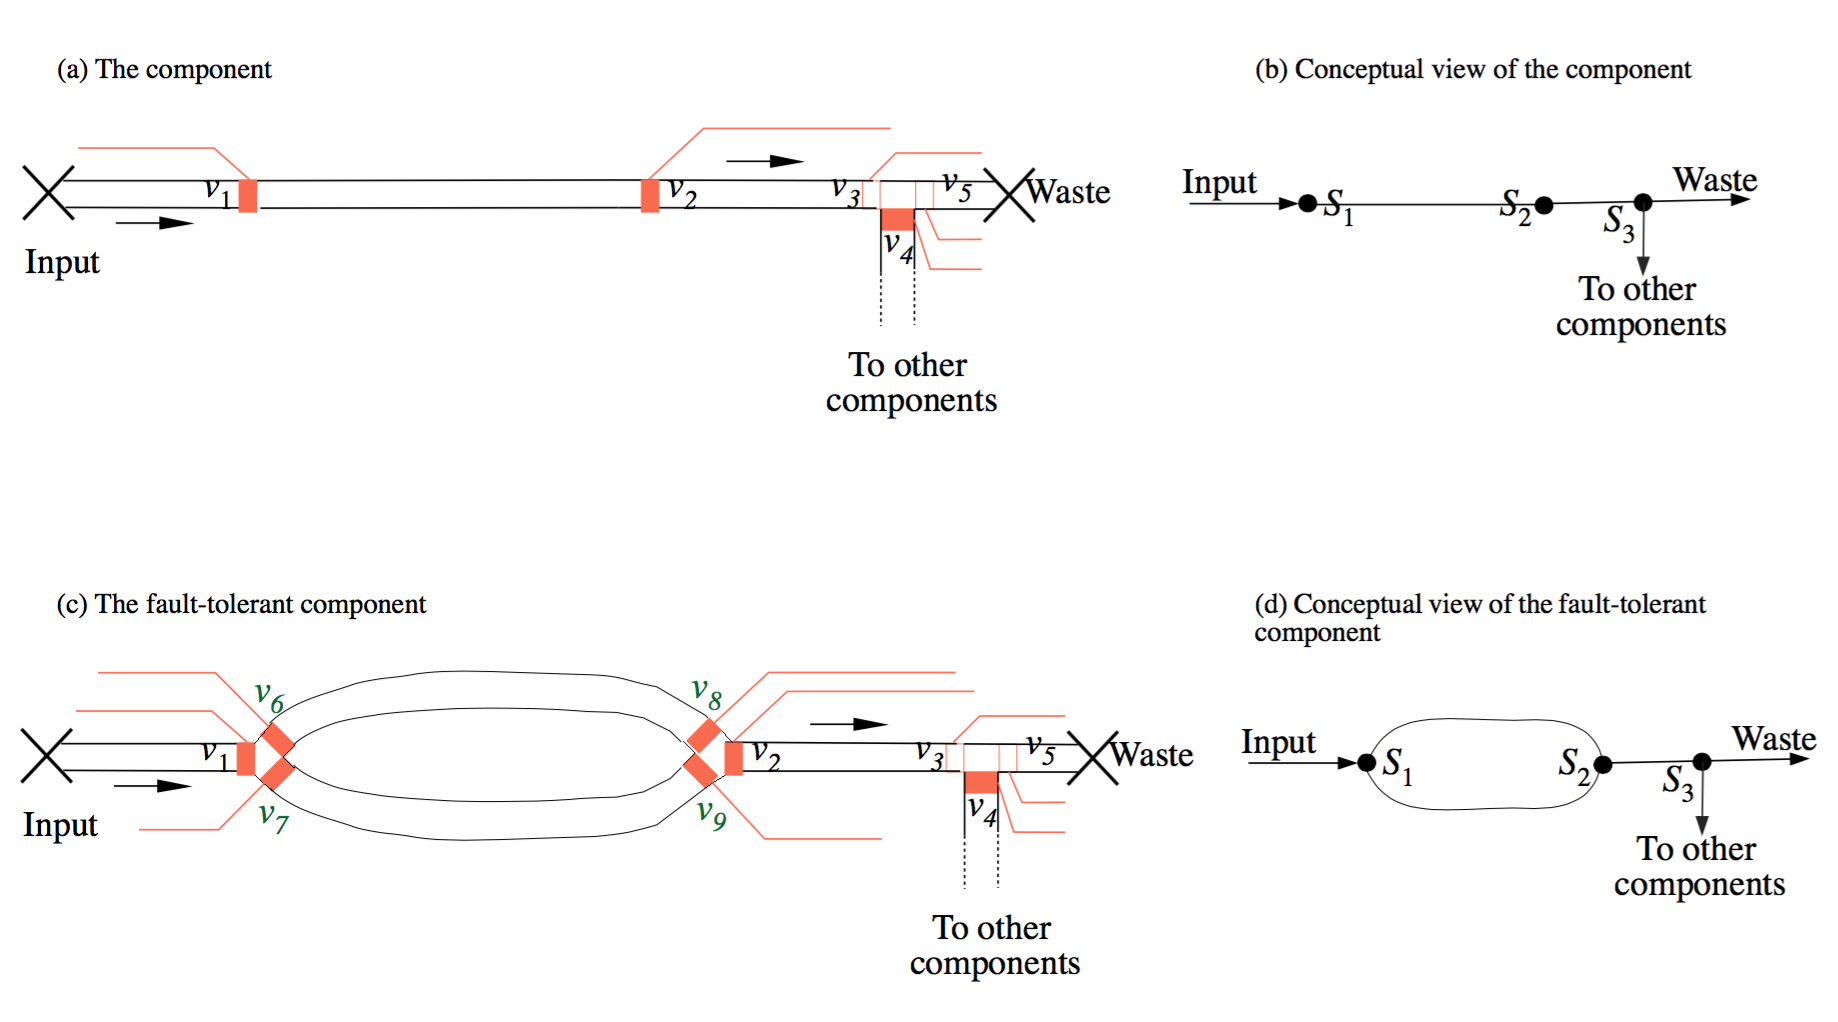
\includegraphics[scale=0.35]{figures/component-and-ftcomponent.png}
\caption[Heater, Filter, Detector and Separator and their fault-tolerant counterpart]{Heater, Filter, Detector and Separator and their fault-tolerant counterpart}
\label{fig:comp-and-ftcomp}
\end{figure}

\autoref{fig:comp-and-ftcomp}a shows a component which consists of two valves $v_1$ and $v_2$. \autoref{fig:comp-and-ftcomp}b shows the conceptual view of the same component. The valve $v_1$ is termed as switch $S_1$ and facilitates the input. The valve $v_2$ is termed as switch $S_2$ and facilitates the output. The two valves also trap the fluid in the channel such that the component-specific operation can take place. The component can fail in various ways. The valves $v_1$ and $v_2$ can either be stuck open or stuck closed. If either valve is stuck open the component cannot trap the fluid as needed by using its valves. If $v_2$ is stuck closed the fluid cannot leave the channel. Additionally if the channel of the component is blocked, the channel is not usable and similarly if $v_1$ is stuck closed the channel is not reachable. Furthermore the channel can also suffer from a leakage.

\autoref{fig:comp-and-ftcomp}c shows a fault-tolerant version of the component which consists of six valves $v_1$, v$_2$, $v_6$, $v_7$, $v_8$ and $v_9$. \autoref{fig:comp-and-ftcomp}d shows the conceptual view of the same fault-tolerant component. The valve set $\{v_1, v_6, v_7\}$ is termed as switch $S_1$ and facilitates the input. The valve set $\{v_2, v_8, v_9\}$ is termed as switch $S_2$ and facilitates the output. The component has two channels, where the fluid can be trapped while the component performs its component-specific operational phase(s). The valve set $\{v_6, v_8\}$ can trap the fluid between them and similarly $\{v_7, v_9\}$. The fault-tolerant component can tolerate one channel suffering from a block defect as it is possible to use the other non-faulty channel. It can also tolerate $v_1$ and $v_2$ being stuck open as the valves are no longer essential for trapping the fluid inside the channels. However, if either $v_1$ or $v_2$ are stuck closed then it is not possible to enter or leave the component, respectively. Therefore, the component would still be considered faulty in the event of these two faults occuring.

\begin{description}
\item[Detector] The channel in a detector acts as a detection channel which identifies and quantifies analyte by various methods. Fluorescence is one among the many techniques to perform detection \cite{component-view}. The fault-tolerant version is called \emph{ft-detector}. The detector and ft-detector have 3 operational phases - Input / Detect / Output.

\item[Heater] The fluid trapped in the heating channel is heated by a metal plate under the flow layer, which is activated when needed. The fault-tolerant version is called \emph{ft-heater}. The heater and ft-heater have 3 operational phases - Input / Heat / Output.

\item[Filter] The channel acts as a filtration channel, which treats and isolates the analyte of interest from crude biological samples. Current methods of filtration include the use of membranes, gels, electrophoresis and dielectrophoresis \cite{component-view}. The fault-tolerant version is called \emph{ft-filter}. The filter and ft-filter have 4 operational phases - Input / Filter / Output1 and Output2.

\item[Separator] The channel acts as a separation channel which isolates samples after other processes. Capillary electrophoresis is a used technique to perform the separation. In this technique, the ionic particles are isolated by their charge and frictional forces \cite{component-view}. The fault-tolerant version is called \emph{ft-separator}. The separator and ft-separator have 5 operational phases - Input1 / Input2 / Separate / Output1 / Output2.

\end{description}


\subsubsection{Fault-tolerant Storage}
\autoref{fig:storage} shows a storage component with eight reservoirs $Res_1$-$Res_8$ and 28 valves total. The storage component is used to store fluid output from chemical or biological reactions on the biochip. The fluid is stored in the channels between the valve sets $\{v_5, v_5\}$ and $\{v_6, v_6\}$. The storage component only receives input or outputs fluid. The storage component can fail in many ways as it has a lot of valves and channels. Each valve in the component can be stuck open or stuck closed or any channel in the component could be suffering from a block defect or leakage. However since the storage component has so many channels and valves it has some fault-tolerance in itself depending how much storage is needed in a given application at the same time. If it is necessary to store four fluids at the same time and four of the storage reservoirs' channel are blocked, then the application can still run.

\begin{figure}[H]
\centering
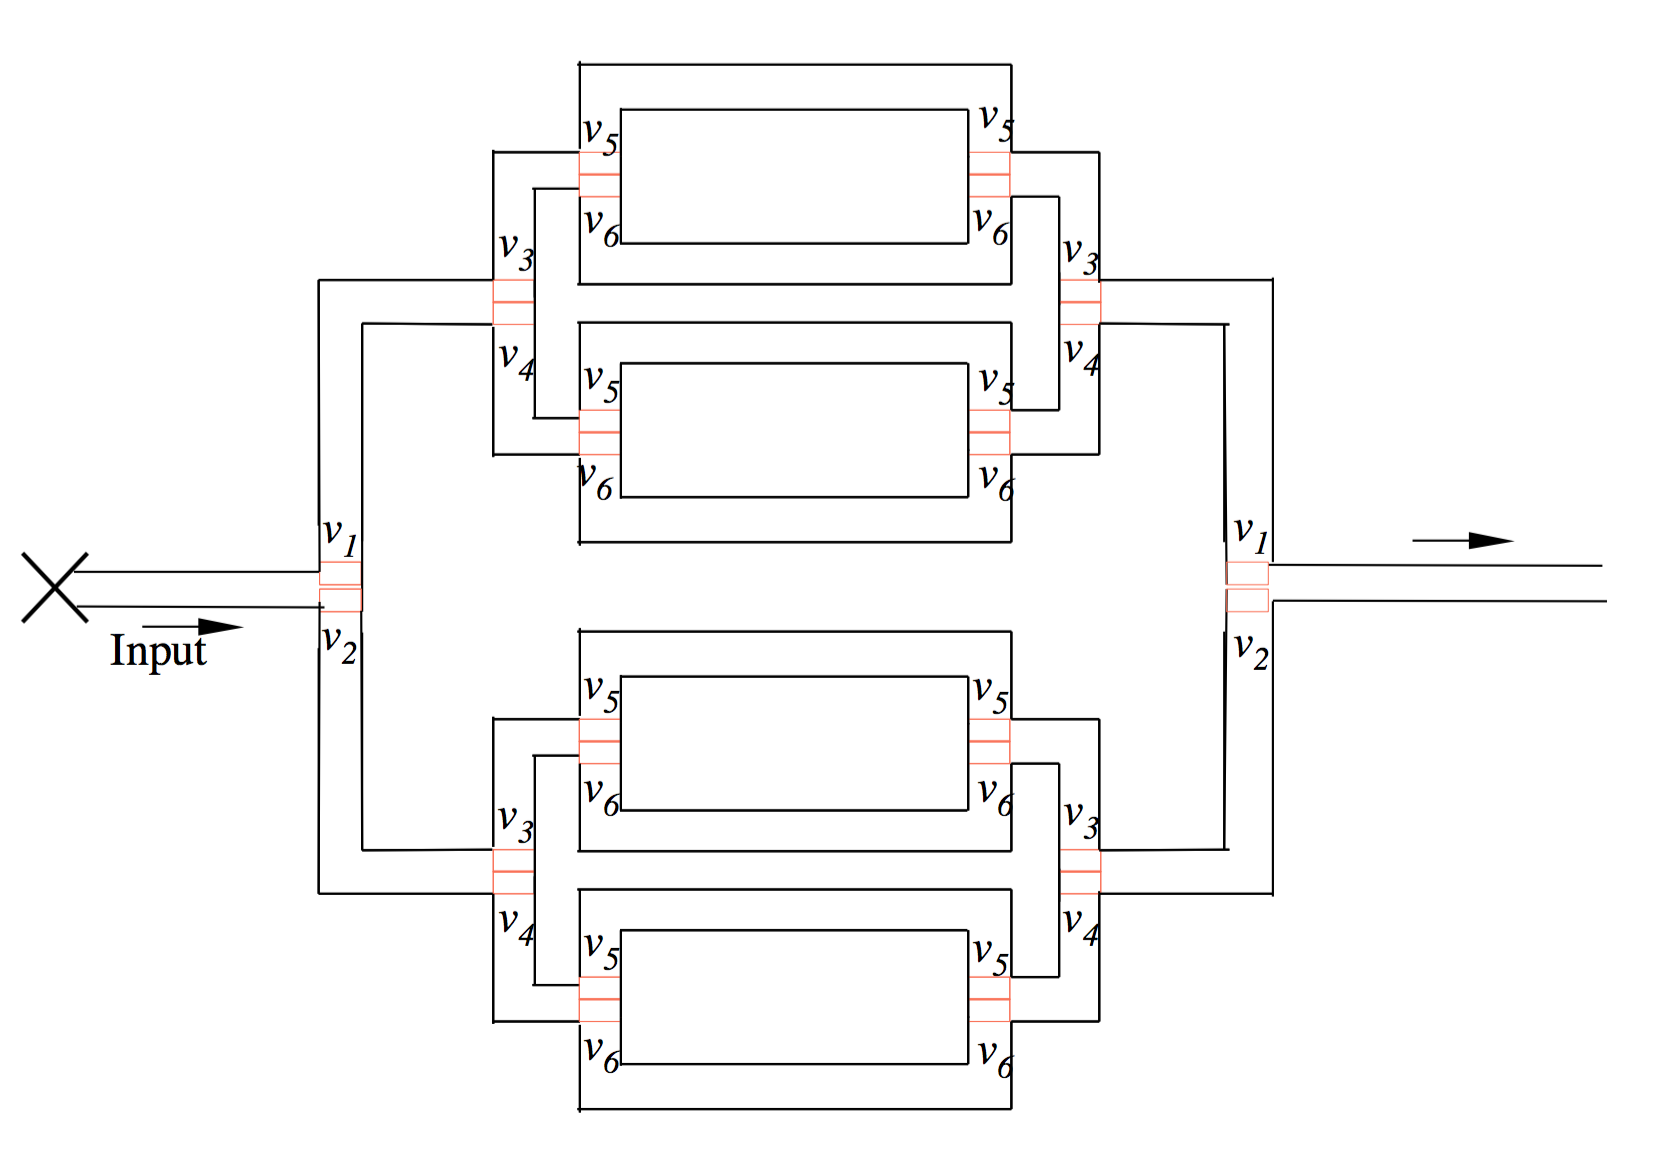
\includegraphics[scale=0.25]{figures/storage-valves.png}
\caption[Storage component]{Storage component}
\label{fig:storage}
\end{figure}

\begin{figure}[H]
\centering
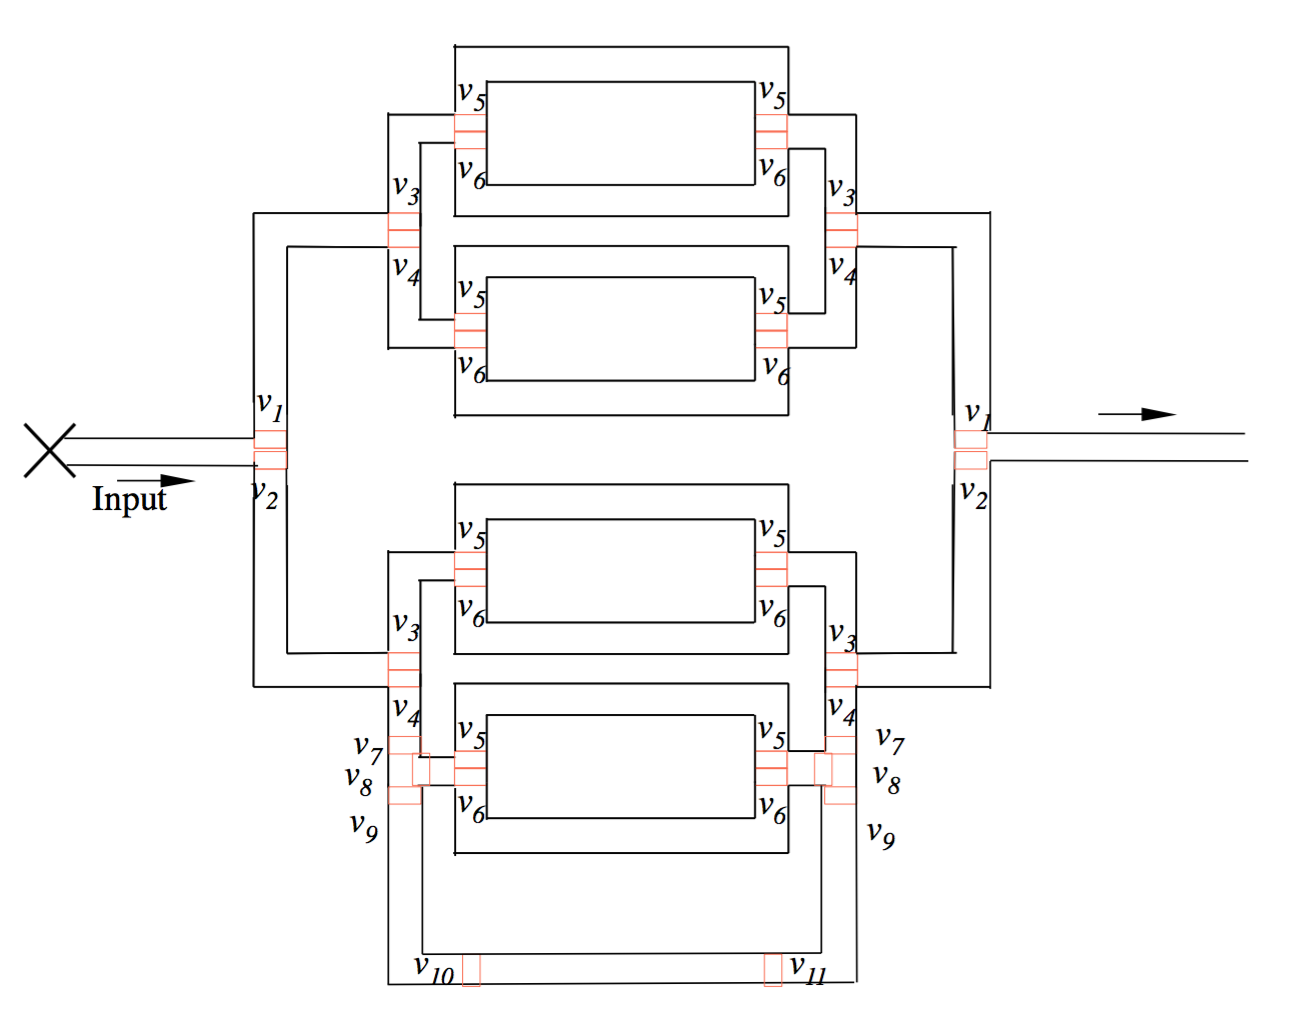
\includegraphics[scale=0.35]{figures/fault-tolerant-storage-valves.png}
\caption[Fault-tolerant storage component]{Fault-tolerant storage component}
\label{fig:ftstorage}
\end{figure}

Additionally, it can also receive input and output from/to both sides and thereby the two channels controlling the input can also be blocked and the storage component is still usable. Furthermore, similar to the mixer, it is possible to route through the storage component as the operations of the storage are performed using only valves and thereby the fluid cannot be unintentionally affected in any way.


\autoref{fig:ftstorage} shows a fault-tolerant version of the storage component with nine reservoirs $Res_1$-$Res_9$ and 34 valves. It is called fault-tolerant storage or \emph{ft-storage} for short. The ft-storage has one more channel to store fluid than the regular storage component, thereby adding additional fault-tolerance to the storage component if there is a need to store eight fluids at the same time and one of the reservoir's channel is blocked.

\subsection{Architecture Model}
\label{sec:arch-model}
The architecture model outlined is proposed in \cite{wajid}. The biochip architecture is modeled by a topology graph $\mathcal{A} = (\mathcal{N}, \mathcal{S}, \mathcal{D}, \mathcal{F}, \mathcal{K}, c)$, where $N$ is a finite set of vertices, $\mathcal{S}$ is a subset of $\mathcal{N}$, $\mathcal{S} \subseteq \mathcal{N}$, $\mathcal{D}$ is a finite set of directed edges, $\mathcal{F}$ is a finite set of flow paths and $\mathcal{K}$ is a finite set of routing constraints. A vertex $N \in \mathcal{N}$ has two distinguished types, a vertex $S \in \mathcal{S}$ represents a switch, whereas a vertex $\mathcal{M} \in \mathcal{N}$, $\notin \mathcal{S}$ represents a component or input/output node. A directed edge $D_{i, j}$ denotes a direct connection from vertex $N_i$ to $N_j$ where $N_i, N_j \in \mathcal{N}$. A flow path, $F_i \in \mathcal{F}$, is a subset of two or more directed edges of D, $F_i \subseteq \mathcal{D}$, $|F_i| > 1$, denoting a direct communication link between two vertices $\in N$ using a chain of directed edges $\in \mathcal{D}$. A routing constraint $K_i \in \mathcal{K}$ is a set of flow paths that are mutually exclusive with the flow path $F_i \in \mathcal{F}$. These flow paths can not be activated in parallel. The function $c(y)$ where $y$ is either a directed edge $D_{i, j} \in \mathcal{D}$ or a flow path $F_i \in \mathcal{F}$ denotes the routing latency, i.e. the time required by a fluid sample to traverse $y$.

\begin{figure}[H]
\centering
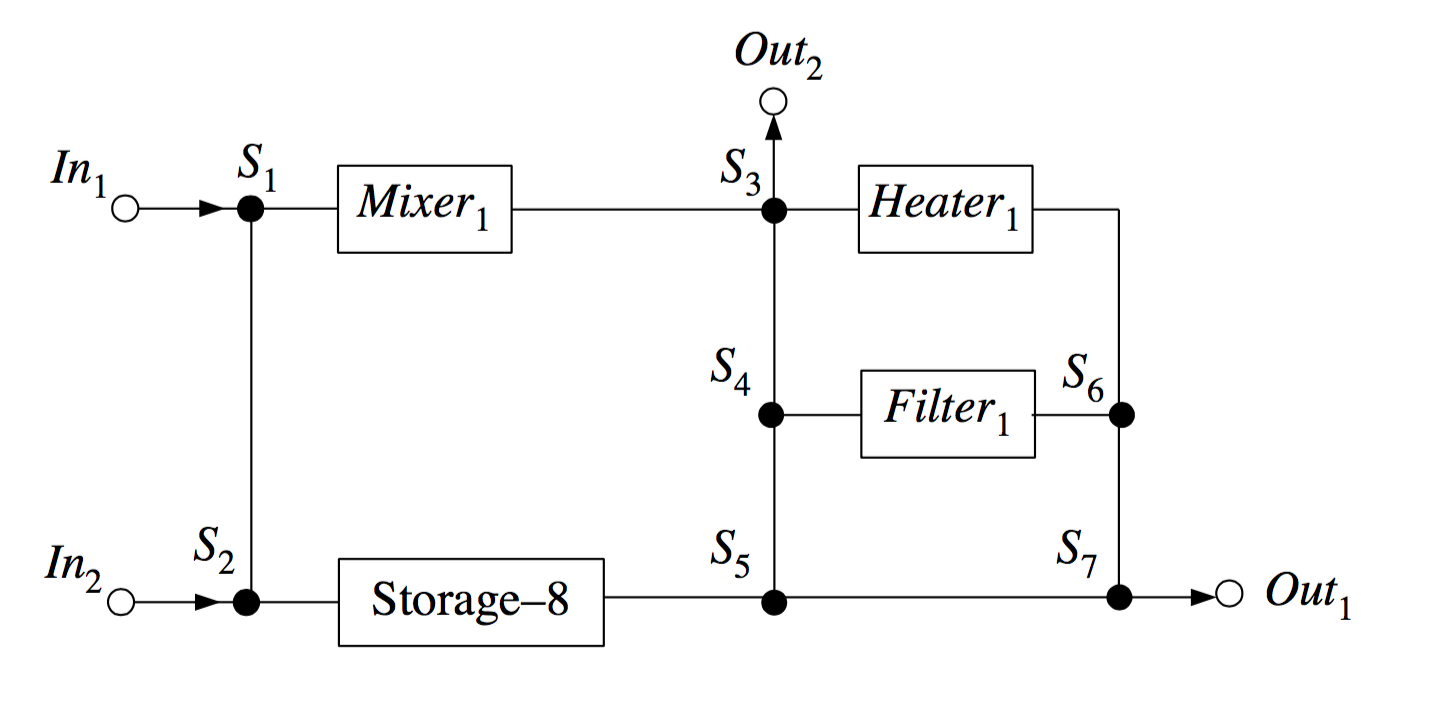
\includegraphics[scale=0.4]{figures/architecture.png}
\caption[Biochip architecture]{Biochip architecture}
\label{fig:architecture}
\end{figure}

\autoref{fig:architecture} shows a biochip architecture equipped with two inputs, two outputs, one mixer, one heater, one filter and eight storage reservoirs $Res_1$-$Res_8$ which are contained in the component 'Storage-8'.

%In this thesis each architecture has a pre-defined average connection time, i.e. each connection in the architecture takes a pre-defined average time to traverse. The exact times are known once the physical routing is done though we do not have that yet.

\subsubsection{Netlist}
The netlist defines which components are to be placed on the biochip and their interconnections. Therefore, it models the functionality of the chip but not the physical layout. The netlist is modeled as a directed graph where components are nodes and the connections between components are the edges, i.e. the nodes are $\mathcal{N}$ from the architecture model and the edges are $\mathcal{D}$.

\subsection{Fault Model}
\label{sec:fault-model}
The following is a proposed fault model for flow-based biochip architectures. The faults are modeled as a set of faults $\mathcal{Z} = (\mathcal{VF}, \mathcal{CF}, v, c)$, where $\mathcal{VF}$ is a finite set of valve faults and $\mathcal{CF}$ is a finite set of channel faults. A valve fault $VF(N, w, t) \in \mathcal{VF}$ can happen to a vertex $N \in \mathcal{N}$ in the architecture. The component model, which specifies the valves, is part of the architecture. The valve affected by the fault is denoted by $w$. The type of fault is denoted by $t$. The type of fault is either stuck open or stuck closed. The $v$ in the fault model specifies the maximum number of valve faults happening at any time in the biochip architecture. Therefore more than $v$ valve faults, $VF \in \mathcal{VF}$, can be specified in the fault model.\\
A channel fault can happen to a component $M \in \mathcal{N}, \notin \mathcal{S}$ in the architecture. A channel fault can also happen to a connection $D_{i, j} \in \mathcal{D}$. The type of fault is denoted by $t$, where the type of fault can either be a block defect or leak. A channel fault on a component is denoted by $CF(M, t) \in \mathcal{CF}$. A channel fault on a connection is denoted by $CF(D_{i, j}, t) \in \mathcal{CF}$. The $c$ in the fault model specifies the maximum number of channel faults happening in the biochip architecture at any point. Hence more than $c$ channel faults, $CF \in \mathcal{CF}$, can be specified in the fault model.

This means that the set of faults in the fault model are divided into two categories - valve faults and channel faults where valves can either be stuck open or stuck closed and channels can either suffer from a block defect or leakage. The set of faults is specific to a biochip architecture. The faults are specific, i.e. when the faults are specified, they denote a specific channel or valve suspected to be faulty. The faults in the fault model can be faults, known by the designer, to be common faults in the architecture.

Considering the architecture in \autoref{fig:architecture} a possible fault model could be: $\mathcal{Z} = (\mathcal{VF}, \mathcal{CF}, 2, 2)$.

\begin{table}[H]
\centering
\caption{Example set of valve faults $\mathcal{VF}$}
\begin{tabular}{| c | c | c | c |}
\hline
\textbf{Name} & \textbf{Vertex} ($N \in \mathcal{N}$) & \textbf{Valve affected} $(w)$ & \textbf{Type} $(t)$ \\ \hline
$VF_1$ & $Mixer_1$ & $v_5$ & Open \\ \hline
$VF_2$ & $S_6$ & $v_3$ & Open \\ \hline
$VF_3$ & $S_5$ & $v_2$ & Open \\ \hline
$VF_4$ & $S_3$ & $v_3$ & Open \\ \hline
\end{tabular}
\label{tab:valve-faults}
\end{table}

\begin{table}[H]
\centering
\caption{Example set of channel faults $\mathcal{CF}$}
\begin{tabular}{| c | c | c | c |}
\hline
\textbf{Name} & \textbf{Component} ($M \in \mathcal{N}, \notin \mathcal{S})$ \textbf{/} \textbf{Connection} $D_{i, j} \in \mathcal{D}$ & \textbf{Type} $(t)$ \\ \hline
$CF_1$ & $Heater_1$ & Block \\ \hline
$CF_2$ & $Filter_1$ & Block \\ \hline
$CF_3$ & $S_2 \rightarrow$ Storage-8 & Block \\ \hline
$CF_4$ & $S_1 \rightarrow Mixer_1$ & Block \\ \hline
\end{tabular}
\label{tab:channel-faults}
\end{table}

A possible fault scenario using this fault model example could be the combination $\{VF_1, VF_3, CF_1, CF_3\}$. In this scenario these four faults are considered to be affecting the architecture. This fault scenario has a lot of effects on the architecture. $CF_3$ specifies that the connection from $S_2 \rightarrow$ Storage-8 is blocked and therefore reaching the Storage-8 component from $In_2$ a longer route is necessary going through $S_1$, $Mixer_1$, $S_3$, $S_4$, $S_5$ and then reaching Storage-8. $VF_1$ effectively means that $Mixer_1$ is faulty and cannot perform its mixing operation as valve $v_5$ (in the pump) is stuck open, however it is still possible to route through $Mixer_1$. $CF_1$ means that the $Heater_1$ is suffering from a block defect and therefore the channel is not usable which renders $Heater_1$ faulty. $VF_3$ specifies that $v_2$ of $S_5$ is stuck open and therefore when reaching $S_5$ in the architecture the routing possibilities depend on which channel is used to enter the switch. Valve $v_2$ restricts / allows the flow to channel between $S_5$ and Storage-8. Therefore, if $S_5$ is entered from Storage-8 the fluid can leave $S_5$, using any other channel. However, if $S_5$ is entered from any other channel it can only use the channel going to Storage-8.\\

A fault scenario is a combination of faults, where any combination of the faults specified in the fault model is possible to create a fault scenario. The defects in the biochip architecture are tested for and known after fabrication. Effectively, this eliminates the tolerance of faults presented at run-time. A valve stuck closed and a blocked channel fault lead to the same result as the channel cannot be used since the valve controls the input and/or output of the channel.

\section{Biochemical Application Model}
\label{sec:app-model}
The biochemical application model outlined is proposed in \cite{wajid}. The biochemical application is modeled by a sequencing graph. The graph $\mathcal{G}(\mathcal{O}, \mathcal{E})$ is directed, acyclic and polar. Therefore, the graph will always have a source vertex with no predecessors and a sink vertex with no successors. Each vertex $O_i \in \mathcal{O}$ represents an operation in the biochemical application. The dependency constraints in the assay are modeled by the edge set $\mathcal{E}$. An edge $e_{i, j}$ from $O_i$ to $O_j$ describes that the output of $O_i$ is the input of $O_j$. All the inputs need to arrive before an operation can be activated. The operations in the application can be bound to a component by the binding function: $\mathcal{B} : \mathcal{O}  \rightarrow \mathcal{M}$. Each vertex has an associated weight $C^{M_j}_i$. This denotes the execution time required for operation $O_i$ to be completed on component $M_j$. The application is assumed to have a deadline which it should complete within. This deadline is denoted as $d_\mathcal{G}$. Furthermore it is also assumed that the biochemical application has been correctly designed, i.e. all the operations will have the correct volume of liquid available for their execution.

\begin{figure}
\centering
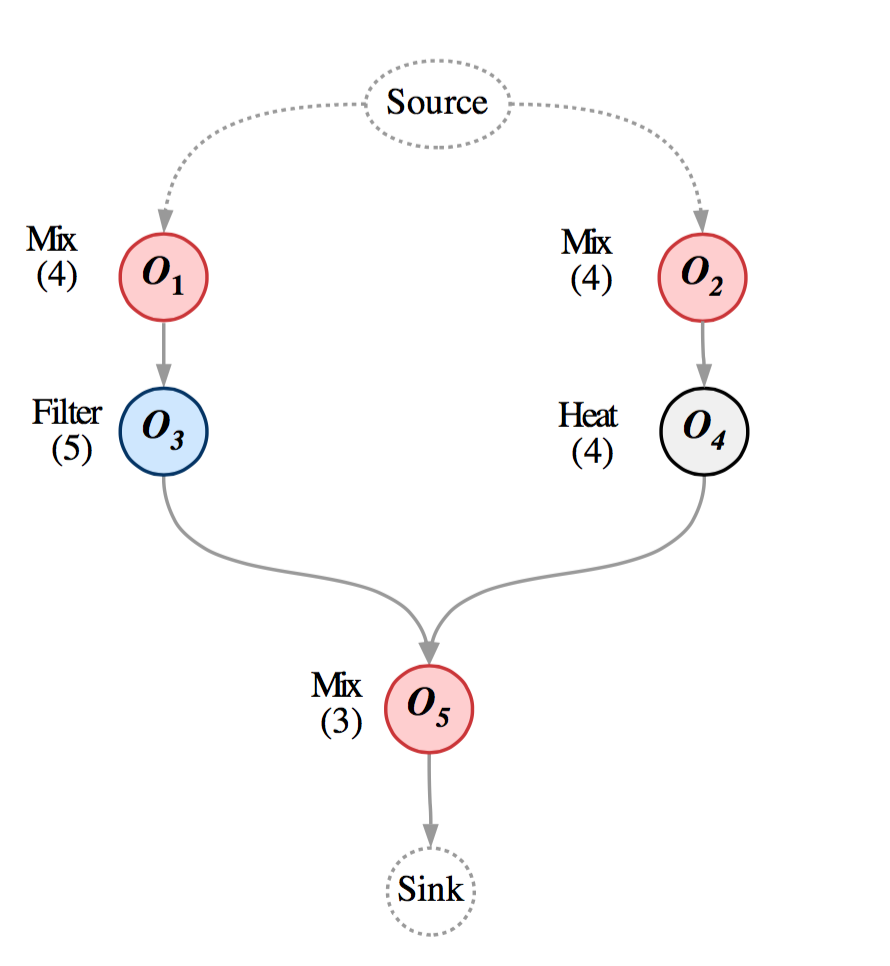
\includegraphics[scale=0.4]{figures/application-model.png}
\caption[Application model]{Application model}
\label{fig:application}
\end{figure}

\autoref{fig:application} shows a simple application model that has 3 mixing operations ($O_1$, $O_2$ and $O_5$), 1 filtration operation ($O_3$) and 1 heating operation ($O_4$). The execution times for each operation are given in the parameter below the operation type. The execution times provided in \autoref{tab:component-library}, are of the actual functional phase, which is given in bold in the table. The execution times from this table are the typical execution times for the component types, however a biochemical application description may specify a longer time, if required for a particular operation.


\section{Application Mapping}
\label{sec:app-map}
Application mapping is the problem of mapping a biochemical application onto a given biochip architecture. Mapping the application onto the architecture involves \emph{binding} onto the allocated components, \emph{scheduling} the operations and performing the required fluidic \emph{routing}. The architecture is modeled as described in \autoref{sec:arch-model} and the application is modeled as outlined in \autoref{sec:app-model}. The allocated components are therefore captured by the vertex set $\mathcal{M}$, $\mathcal{M} \in \mathcal{N}$, in the architecture model $\mathcal{A}$. The component placement and interconnections are also captured in the topology graph $\mathcal{A}$ modeling the architecture.\\
During the binding step, each vertex $O_i$, $O_i \in \mathcal{O}$, representing a biochemical operation in the application model is bound to an available component $M_j$, i.e. $\mathcal{B}(O_i) = M_j$. Since the fluid transport latencies in microfluidic chips are comparable to the operation execution times, fluid routing also needs to be considered. Therefore, the binding function must also capture the binding of the edge set $\mathcal{E} \in \mathcal{G}$ to an available route. The route can be a flow path, $F \in \mathcal{F}$, or a collection of flow paths called a \emph{composite route}. A composite route is used when the source and destination components are such that no direct flow path exists between them.\\
A scheduling strategy is necessary to efficiently execute the biochemical operations on the biochip components, while considering the dependency captured by the application model and the resource constraints captured by the biochip architecture. Alongside, the set of operations $\mathcal{O} \in \mathcal{G}$ given in the application model the edge set $\mathcal{E} \in \mathcal{G}$ also needs to be scheduled on the biochip while considering the routing constraints. Before scheduling a specific edge, the implementation needs to evaluate if a flow path $F \in \mathcal{F}$ is sufficient to bind the edge or if a composite route is necessary.\\
Throughout the scheduling phase, the storage requirement analysis needs to be performed. Consequently, after completion of an operation, a decision on whether the output fluid should be moved to a storage reservoir or not, needs to be made.


%\section{Benchmarks}


\section{Summary}
In this chapter, the used biochip architecture model has been outlined. The biochip architecture model has been proposed before. However there is proposed an addition to the component model in form of an extended component library with fault-tolerant components in the flow layer. Furthermore, a fault model for describing faults in the biochip architecture has been proposed with the distinction between valve faults and channel faults. Lastly, the application model used in the thesis has been defined and the problem of mapping an application model onto a given biochip architecture has been outlined.
